\documentclass[a4paper]{article}

\usepackage[english]{babel}
\usepackage[utf8]{inputenc}
\usepackage{csquotes}
\usepackage{amsmath, latexsym}
\usepackage{graphicx}
\usepackage{tikz}
\usepackage{listings}
\usepackage{verbatim}
\usepackage{bigints}
\usepackage{float}
\usepackage{titling}
\usepackage[percent]{overpic}
\usepackage[para]{footmisc}
\usepackage[colorinlistoftodos]{todonotes}
\usepackage[style=authoryear,sorting=nty,maxcitenames=1]{biblatex}

\title{Spherically symmetric bubble collapse problem}
\author{}
\date{\today}

\begin{document}
\maketitle
\section*{Objective}
The present work aims to compute the minimum distance to place the Kirchhoff control surface from the bubble center. For this, we solve the bubble collapse problem in one dimension, assuming spherical symmetry, and obtain the distance at which the ratio of acoustic pressure and ambient pressure of the fluid $p'/p_0 << 1$. We do the convergence study for the Kirchhoff integral and see if the chosen surface is in the linear acoustic regime.
\section*{Governing equation}
The Compressible Euler equations assuming spherical symmetry for the mulitphase system can be written as
\begin{align}
    (\rho)_t + (\rho u)_r &= \frac{-2\rho u}{r},\\
    (\rho u)_t + (\rho u^2 + p)_r &= \frac{-2\rho u^2}{r}, \\
    (E)_t + ((E + p) u)_r &= \frac{-2(E + p) u}{r},\\
    (\phi)_t + (\phi u)_r &= \phi u_r,
\end{align}
where the equation of state for the mixture is given by 
\begin{align}
    p &= (\gamma - 1)(E - \rho u^2/2) - \gamma P^{\infty},\\    
    \gamma &= 1 + \frac{(\gamma_w - 1)(\gamma_a - 1)}{(1 - \phi)(\gamma_w - 1) + \phi(\gamma_a  - 1)},\\
    P^{\infty} &= \frac{\gamma - 1}{\gamma}\Big( \phi \frac{\gamma_w P^\infty_w}{\gamma_w - 1}  +(1 - \phi)\frac{\gamma_a P^\infty_a}{\gamma_a - 1} \Big). 
\end{align}
\subsection*{Initial condition}
An air bubble of radius $R$ is placed in a water medium, assuming the fluid to be stationary. The initial condition for the primitive variables is given by
\begin{align}
    \rho &= \frac{(\rho_a + \rho_w)}{2} + \frac{(\rho_w - \rho_a)}{2}{\tanh\Big(\frac{r - R}{\epsilon h}}\Big),\\
    u &= 0,\\
    p &= \frac{(p_a + p_w)}{2} + \frac{(p_w - p_a)}{2}{\tanh\Big(\frac{r - R}{\epsilon h}}\Big),\\    
    \phi &= \frac{(\phi_a + \phi_w)}{2} + \frac{(\phi_w - \phi_a)}{2}{\tanh\Big(\frac{r - R}{\epsilon h}}\Big).
\end{align}

\begin{figure}[!h]
\centering
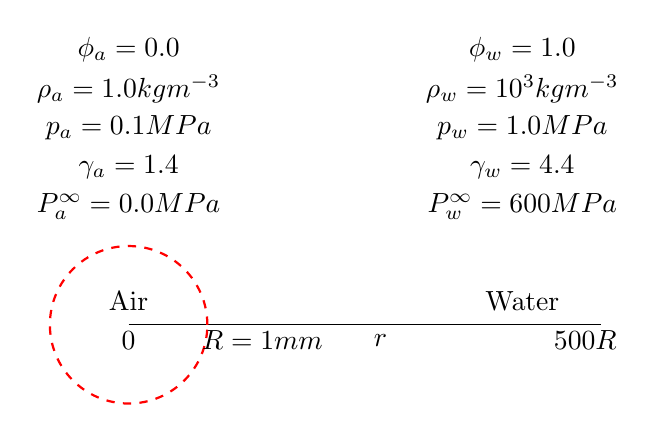
\begin{tikzpicture}
    \draw (0, 0) -- (6.0,0);
    \draw [red, thick, dashed] (0, 0) circle (1);
    \draw (1.7, -0.2) node {$R = 1mm$};
    \draw (3.2, -0.2) node {$r$};
    \draw (5.8, -0.2) node {$500R$};
    \draw (0.0, 0.3) node {Air};
    \draw (5.0, 0.3) node {Water};
    \draw (0.0, -0.2) node {0};
    \draw (0.0, 3.5) node {$\phi_a = 0.0$};
    \draw (0.0, 3.0) node {$\rho_a = 1.0 kgm^{-3}$};
    \draw (0.0, 2.5) node {$p_a = 0.1 MPa$};
    \draw (0.0, 2.0) node {$\gamma_a = 1.4$};
    \draw (0.0, 1.5) node {$P^{\infty}_a = 0.0 MPa$};
    \draw (5.0, 3.5) node {$\phi_w = 1.0$};
    \draw (5.0, 3.0) node {$\rho_w = 10^3 kgm^{-3}$};
    \draw (5.0, 2.5) node {$p_w = 1.0 MPa$};
    \draw (5.0, 2.0) node {$\gamma_w = 4.4$};
    \draw (5.0, 1.5) node {$P^{\infty}_w = 600 MPa$};
\end{tikzpicture}
\caption{Schematic of air bubble in water medium with the initial conditions.}
\end{figure}

\subsection*{Boundary condition}
We enforce homogeneous Neumann boundary condition at both ends of the domain $\frac{\partial(*)}{\partial r}\Big |_0 = \frac{\partial(*)}{\partial r}\Big |_L = 0$.

\subsection*{Scaling}
Let $\bar{p}$ be the pressure scale, $\bar{\rho}$ be the density scale and $\bar{x}$ be the length scale. Then
\begin{equation}
    p = \bar{p}p_s, \;\;\;\; \rho = \bar{\rho} \rho_s, \;\;\;\; x = \bar{l}x_s. 
\end{equation}
Where $p_s, \rho_s$ and $x_s$ are the scaled pressure, density and length. We can obtain the velocity and time scale from the above scales.
\begin{equation}
    \frac{M}{LT^2} = \bar{p}\frac{M_s}{L_sT^2_s}, \;\;\;\; \frac{M}{L^3} = \bar{\rho}\frac{M_s}{L^3_s}.
\end{equation}
From the above relations we can obtain,
\begin{equation}
    \frac{L}{T} = \sqrt{\frac{\bar{p}}{\bar{\rho}}}\frac{L_s}{T_s}
\end{equation}
Therefore the velocity and time scale is given by
\begin{equation}
    v = \sqrt{\frac{\bar{p}}{\bar{\rho}}} v_s, \;\;\;\; t = \bar{l} \sqrt{\frac{\bar{\rho}}{\bar{p}}} t_s. 
\end{equation}
For the bubble problem we use the following scales,
\begin{equation}
    \bar{p} = 10^6Pa, \;\;\;\; \bar{\rho} = 1000 kgm^{-3}, \;\;\;\; \bar{l} = 10^{-3} m.
\end{equation}
The scaled initial conditions are
\begin{figure}[!h]
    \centering
    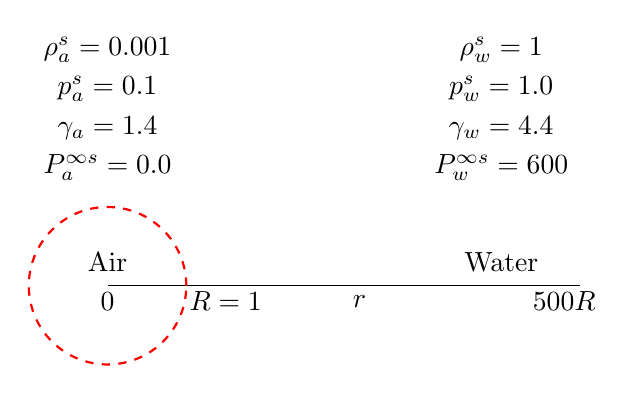
\begin{tikzpicture}
        \draw (0, 0) -- (6.0,0);
        \draw [red, thick, dashed] (0, 0) circle (1);
        \draw (1.5, -0.2) node {$R = 1$};
        \draw (3.2, -0.2) node {$r$};
        \draw (5.8, -0.2) node {$500R$};
        \draw (0.0, 0.3) node {Air};
        \draw (5.0, 0.3) node {Water};
        \draw (0.0, -0.2) node {0};
        \draw (0.0, 3.0) node {$\rho_a^s = 0.001$};
        \draw (0.0, 2.5) node {$p_a^s = 0.1 $};
        \draw (0.0, 2.0) node {$\gamma_a = 1.4$};
        \draw (0.0, 1.5) node {$P^{\infty s}_a = 0.0$};
    
        \draw (5.0, 3.0) node {$\rho_w^s = 1$};
        \draw (5.0, 2.5) node {$p_w^s = 1.0 $};
        \draw (5.0, 2.0) node {$\gamma_w = 4.4$};
        \draw (5.0, 1.5) node {$P^{\infty s}_w = 600 $};
    \end{tikzpicture}
    \caption{Schematic of air bubble in water medium with the scaled initial conditions.}
    \end{figure}
\subsection*{Numerical method}
We use the the minmod reconstruction for the spatial discretization and LLF path conservative Riemann solver for the flux computation. The time integration is done using the SSPRK22 method. The cell size is chosen $h = 0.01$ to resolve the bubble with $100$ cells per bubble radius and the time step is computed based on CFL $= 0.8$.

\subsection*{Keller-Miksis model}
We compare the bubble radius from the numerical solution of the multiphase Euler equation with the Keller-Miksis model. The Keller-Miksis model is an ordinary differential equation describing the time evolution of the bubble radius
\begin{equation}
   \Bigg( 1 - \frac{\Dot{R}}{c_\infty} \Bigg)R \Ddot{R} + \frac{3}{2} \Bigg(1 - \frac{\Dot{R}}{3c_\infty} \Bigg)\Dot{R}^2 = \frac{1}{\rho_\infty} \Bigg( 1 + \frac{\Dot{R}}{c_\infty} + \frac{R}{c_\infty}\frac{d}{dt}\Bigg)(p - p_\infty).
\end{equation}
Where,  $p$ is the bubble wall pressure given by
\begin{equation}
    p = p_{\infty} \Bigg( \frac{R_0}{R} \Bigg)^{3 \kappa}, \;\;\; \kappa = 1.4 
\end{equation}
\begin{figure}[h!]
    \centering
    \includegraphics[scale=0.7]{images/kellermiksis.png}
    \caption{Time evolution of the bubble radius obtained from solving the multiphase Euler equation compared with the Keller-Miksis model.}
\end{figure}
\subsection*{Acoustic pressure ratio at various distances}
We extract the acoustic pressure at various distances from the center of the bubble and find the maximum norm of ratio of acoustic pressure and ambient pressure of the fluid $\Big|\frac{(p - p_w)}{p_w} \Big |$.
\begin{table}[h!]
    \begin{tabular}{c c}
        $R/R_0$ & $max \Big|\frac{(p(t) - p_w)}{p_w} \Big |$ \\
        $10$ & $3.97e-1$ \\
        $50$ & $7.95e-2$ \\
        $100$ & $2.88e-2$ \\
        $250$ & $1.15e-2$ \\ 
        $300$ & $9.58e-3$ \\
        $450$ & $6.38e-3$ \\
    \end{tabular}
\end{table}
We keep the control surface at different distances and check the convergence of Kirchhoff integral.
\subsection*{Convergence of Kirchhoff integral}
\begin{figure}[!h]
    \centering
    \begin{tikzpicture}
        \draw (0, 0) -- (9.0,0);
        \draw [red, thick, dashed] (0, 0) circle (1);
        \draw [blue, thick, dashed] (0, 0) circle (3);
        \draw (1.5, -0.2) node {$R = 1$};
        \draw (3.2, -0.2) node {$R_{k}$};
        \draw (9.0, -0.2) node {$500R$};
        \draw [red, thick, fill] (7, 0.0) circle (0.05);
        \draw (7, -0.2) node {$R_{o} = 450R$};
        \draw (0.0, 0.3) node {Air bubble};
        \draw (3.2, 2.0) node {Kirchhoff surface};
        \draw (5.0, 0.3) node {Water};
        \draw (0.0, -0.2) node {0};
       
     \end{tikzpicture}
    \caption{Schematic of Kirchhoff control surface and far-field observer point}
\end{figure}
We compute the Kirchhoff integral
\begin{equation}
    \begin{split}
        p'(r,t) =  \frac{1}{4\pi}\int_{0}^{2\pi}\int_{0}^{\pi}\Big[  \frac{p'}{r'^{2}}&\frac{\partial r'}{\partial n} - \frac{1}{r'}\frac{\partial p'}{\partial n} + \frac{1}{c r'}\frac{\partial r'}{\partial n}\frac{\partial p'}{\partial \tau} \Big]_{\tau} R^2\sin\theta d\theta d \phi  
    \end{split} 
\end{equation}
using the mid-point rule and obtain the acoustic pressure at the observer point.
\begin{figure}[h!]
    \centering
    \includegraphics[scale=0.7]{images/Convergence.png}
    \caption{\textcolor{red}{We did not obtain the expected second-order convergence for the Kirchhoff integral.}}
\end{figure}



\end{document}
